\chapter{Quantum Error Correction Codes.}
\section{Introduction.}
It's widely believed that quantum machines have a significant advantage over the classical in the range of computational tasks\cite{grover1996fast}, \cite{ahuja1999quantum}. Simple algorithms could be interpreted as the quantum version of scanning all the options, cutting the running time by the square root of the classical magnitude. 

Nevertheless, Shore has shown a polynomial depth quantum circuit that solves the hidden abelian subgroup \cite{Shor_1997}, which is considered a breakthrough, as it made the computer science community believe that a quantum computer might offer an exponential advantage.

Yet, even though there is a consensus about the superiority of ideal quantum computation model, it is still unclear whether implementing such a machine in the presence of noise is feasible.   
Still, just pointing on the existence of noise is not powerful enough to cancel the feasibility of computation. Evidence of this is that classical computers also suffer from a certain rate of faults. Thus, to fully understand the hardness, let us compare two main reasons that made it realize a hard task. 
First is the magnitude of the error rate, classical computers also have errors, and sometimes we witness system failures (blue screen, for example). The error rate of modern computers is so low that the probability for error to propagate stays negligible even if the length of the computation is polynomial in the scale of what is considered reasonable input size. It's worth mentioning that in exascale computing when supercomputers perform around $10^{18}$ operations per second, It is hard to miss the faults. In quantum, we become aware of their existence much earlier.      

The second difference, which is a tricky point, is that quantum states are sensitive to additional types of error. Along with the chance for bit-flip error, a quantum state might also change its phase. For example, consider the initial state $\ket{+} = \frac{1}{\sqrt{2}}\left( \ket{0} + \ket{1} \right)$, and suppose that due to noise the state transformed into $\frac{1}{\sqrt{4}}\left( \sqrt{3}\ket{0} + \ket{1} \right)$. While classical circuits are blind to such faults. Namely, their run would stay identical as no error occurs. Quantum circuits usually would affect and might fail. Furthermore, when planning a decoder for quantum error correction codes, If one is willing to use a classical code to defend against phase flips, he has to ensure that the decoding doesn't cause bit-flip errors. 


\ifdefined\qnoise
  \begin{document}
\fi
\section{Quantum Noise.} 
\begin{definition}[Bit and pahse flip.] \label{def:bphf}  
  Consider a quantum state $\ket{\psi}$ encoded in the computation base. We will say that a \textit{bit-flip} occurs in a scenario the operator Pauli $X$ is applied on one of our state's qubits. The bit-flip event could be considered as exactly as the standard bit-flip error in the classical regime. Similarly, \textit{phase-flip} occurs when the Pauli $Z$ is applied on one of the qubits. 

  \end{definition}

  % Notice that together with the identity $I$, the set $\{I, X \otimes e_{i} , Z \otimes e_{j} \}_{i,j \in [n]}$ span the matrices act on $n$ qubits.  


\ifdefined\qnoise
  \end{document}
\fi
 
However, even though quantum noise is so violent, It was proven that any ideal circuit at polynomial depth could be transformed to a robust circuit at poly-logarithmic cost \cite{aharonov1999faulttolerant}. Or in other words, There is a threshold, If the physicists would provide qubits and a finite gate set that suffers from a rate of noise below that threshold, then $BQP$, the class of polynomial time ideal quantum computation is feasible and could be computed on a realistic machine.                

The basic ingredient in \cite{aharonov1999faulttolerant} was to show the existence of quantum error correction code, such that one can perform all the logic operations in a way that restricts present errors from propagating on. That allows them to separate any operation of the computation into stages; one of them is the operation itself, another one is an error correction stage. That process comes with an additional cost, in both space and time, yet it might decrease the probability that the final state at the end would be faulted. The trade-off between the resource needed to pay and the decreasing rate defines the threshold. And if the balance is positive, then one can repeat in a recursion manner, and after log-log iterations, the failure probability decay to zero. At the same time, the circuit would scale at most poly-logarithmic wide and depth factors.      

Let's return to the repetition code presented in Chapter 2. We would like to have an analog; a first and natural attempt might consider duplicating copies of the state. Unfortunately, copying a general state is not a linear operation and therefore can not be done in the circuit model (and any other believed to be feasible). In particular there is no circuit $U$ which duplicate simultaneity the states $\ket{0}, \ket{1}, \ket{+}, \ket{-}$.

To overcome the issue, Shor came up with the nine-quibt code \cite{Ninequ}, which at first glance might seem a naive straightforward implantation of ``duplication'', but instead uses a clever insight about quantumness in general. Any operation can be seen as a linear (and even unitary) operation over a subspace embedded in large enough dimensions. The encoding is given as follow: 
\begin{equation*}
  \begin{split}
    |\overline{0}\rangle&=\frac{1}{2\sqrt{2}}\left(|000\rangle+|111\rangle\right)^{\otimes3}\\
    |\overline{1}\rangle&=\frac{1}{2\sqrt{2}}\left(|000\rangle-|111\rangle\right)^{\otimes3}~.
  \end{split}
\end{equation*}


For convenient let us use the notation, $\ket{\mathbf{GHZ}^{\pm}} =  \ket{0^{m}} \pm  \ket{1^{m}}$. One can also consider the Shor code over $m^{2}$ qubits which defined as above beside that any logical state contain $m$ product over $m$ qubits, So the state $\ket{\overline{0}}$ over $m^{2}$ qubits can be written as $\ket{\mathbf{GHZ}^{+}}^{m}$. We are now ready to prove a statement regards to the robustness.  

\begin{lemma}
  The Shor code over $9$ qubits enable to correct a single either bit or phase flip.  
\end{lemma}
It is evident that a single bit-flip error can be handled in the same way as in the conventional case. The decoder will check if any of the triples have the same value, and if not, it will correct it by majority. To create a decoder that can also correct a phase-flip error, we need the following statement. In this chapter, we denote the Hadamard gate over $m$ qubits as $H^m$.
\begin{claim}
   $H^{m}\ket{\mathbf{GHZ}^{\pm}} = \sum_{ x \cdot \mathbf{1} =_2 \pm }{\ket{x} }$
\end{claim}

\begin{proof}

  \begin{equation*}
    \begin{split}
      H^{m}\ket{\mathbf{GHZ}^{\pm}} & = H^{m}\ket{0^{m}} \pm  H^{m}\ket{1^{m}} = \sum_{x \in \mathbb{F}_{2}^{m}}{\ket{x}} \pm  \sum_{x \in \mathbb{F}_{2}^{m}}{\left( -1 \right)^{x \cdot \mathbf{1}} \ket{x}} \\ & = \sum_{x \in \mathbb{F}_{2}^{m}}{ \left( 1 \pm \left( -1 \right)^{x \cdot \mathbf{1}}  \right) \ket{x} } =  \sum_{x \cdot \mathbf{1} =_2 \pm }{\ket{x} }
    \end{split}
  \end{equation*}
\end{proof}

Now it is clear how to correct a phase flip. One can apply the Hadamard transform and compute the parity of each triple. By the assumption that only a single phase flip may occur, either all the triples have the same parity or the faulted one has an opposite parity and needs to be corrected. Thus, we obtain an $\left[ \left[ 9,1,3 \right] \right]$ quantum error correction code. Asymptotically, this is an $\left[ \left[ m^{2}, 1, m \right] \right]$ code.

\section{CSS Codes.}

The Shor code is a specific case of the more general CSS (Calderbank-Shor-Steane) code \cite{Calderbank_1996}. A family composed by two binary codes $C_{X}, C_{Z}$ such that $C_{Z}^{\perp} \subset C_{X}$. 

\ifdefined\CSSDOC
\begin{document}
\fi 

\ctt{Add a definition of error weight. fault that spanned by pauli operator of degree at} 

\begin{definition}[CSS Code]
  Let $C_{X}, C_{Z}$ classical linear codes such that $C_{Z}^{\perp} \subset C_{X}$ define the $Q\left( C_{X},C_{Z} \right)$ to be all the code words with following structure:
  \begin{equation*}
    \begin{split}
    \ket { \mathbf{ x } } := \ket { x + C_{Z}^{\perp} } = \frac{1}{\sqrt{C_{Z}^{\perp}}} \sum_{z \in C_{Z}^{\perp}}{ \ket{ x + z }} 
    \end{split}
  \end{equation*}
\end{definition}
Clearly, the codewords are all the codewords in $C_{X}$ which don't belong to $C_{Z}^{\perp}$ and therefore the dimension of the quantum code is $\dim Q\left( C_{X}, C_{Z} \right) = \dim C_{X} - \dim C_{Z^{\perp}} = \dim C_{X} + \dim C_{Z} - n$. Yet, it's not stems immediately how one can correct faults. Next, we are going to repeat the decoding process of the Shor code in the general setting of CSS codes.  
\begin{lemma}
  Let $C_{X},C_{Z}$ classical codes such $Q\left( C_{X},C_{Z} \right)$ is a CSS code. Let $d_{X}$ be the minimal weigh of codeword in $C_{X}$ which is not in $C_{Z}^{\perp}$, and define by the same way $d_{Z}$ to be the minimal weight of codeword in $C_{Z}$ which doesn't belong to $C_{X}^{\perp}$. Then the distance of $Q\left( C_{X},C_{Z} \right)$ equals to $\min{d_{X},d_{Z}}$. Moreover there is a decoder which correct any fault with weight at most $d/2$.       
  \end{lemma}

    \newcommand{\GZZZ}[1]{ \frac{1}{\sqrt{|C_{Z}^{\perp}|}} \sum_{z \in C_{Z}^{\perp}}{ #1 } } 
    \newcommand{\GZZZW}[2]{ \frac{1}{\sqrt{|C_{Z}^{\perp}|}} #2 \sum_{z \in C_{Z}^{\perp}}{ #1 } } 
    \newcommand{\GXXX}[1]{ \frac{1}{\sqrt{|C_{Z}|}} \sum_{z \in C_{Z}}{ #1 } } 
    \newcommand{\GXXXW}[2]{ \frac{1}{\sqrt{|C_{Z}|}} #2 \sum_{z \in C_{Z}}{ #1 } } 

  \begin{proof}
    First let us prove the following claim: 
    \begin{claim}
      Denote by $H^{\otimes n}$ the Hadamard gate over $n$ qubits. Then for any code $C$ it holds that: $  H^{n}\ket{C^{\perp}} = \ket{C} $
          \end{claim}
    \begin{proof}
      \begin{equation*}
        H^{n}\ket{C^{\perp}} = \GZZZ{ H^{n}\ket{z} } = \frac{1}{ \sqrt{ 2^{n}}} \GZZZ{ \sum_{y\in \mathbb{F}_{2}^{n}}{ (-1)^{\braket{z,y}}  \ket{y}}  }
       \end{equation*}
       Notice that $ 2^{n}|C_{Z}^{\perp}| =  |C_{z}| \cdot |C_{Z}^{\perp}| \cdot |C_{Z}^{\perp}|$  
    \end{proof}
    \begin{claim}
      For any $x_{0} \in C_{X}$ and $z_{1}\neq z_{2} \in C_{z}^{\perp}$, $D$ correct $\ket{x+z_{1}+f}$, $\ket{x+z_{2}+f}$ into two different words in $C_{X}$. 
    \end{claim} 
    \begin{proof}
      Suppose not, namely there exists $y \in C_{X}$ such that $D$ correct $\ket{x+z_{1}+f}$, $\ket{x+z_{2}+f}$ into $\ket{y}$. Then we have that for both $i\in \{1,2\}$ it holds that  $d\left( x+z_{i} +f, y \right) \le d\left( C_{Z}^{\perp}/2 \right)$ and therefore $ d\left( x + z_{1} + f, x+z_{2} +f  \right) \le d\left( C_{Z}^{\perp} \right)$. But
      \begin{equation*}
        \begin{split}
            & d\left( x + z_{1} + f, x+z_{2} +f  \right) =  | x + z_{1} + f + x + z_{2} + f | \\
            =  & | z_{1} + z_{2} | = d\left( z_{1},z_{2} \right) > d\left( C_{Z}^{\perp} \right) 
        \end{split}
      \end{equation*}     
      contradiction for the assumption that $z_{1},z_{2} \in C_{Z}^{\perp}$.   
    \end{proof}
    Let $P = X^{f}Z^{e}$ be an error such that $e, f < d/2$ act on the state $\ket{\mathbf{x}}$. Denote by $H_{X}, H_{Z}$ the parity check matrices of $C_{X},C_{Z}$. 
      \begin{equation*}
      \begin{split}
        \ket{\mathbf{x}} &  \mapsto^{P}   \frac{1}{\sqrt{|C_{Z}^{\perp}|}} \sum_{z \in C_{Z}^{\perp}}{ X^{f}Z^{e}\ket{ x + z }} = \frac{1}{\sqrt{|C_{Z}^{\perp}|}} \sum_{z \in C_{Z}^{\perp}}{ (-1)^{\braket{e,f} }Z^{e}\ket{ x + z + f}}\\
        & \mapsto^{H_{X}} \GZZZ{ (-1)^{\braket{e,f} }Z^{e}\ket{ x + z + f} \ket{ H_{X} \left(x + z + f\right) }  } \\ 
        & = \ \ \ \ \ \GZZZ{ (-1)^{\braket{e,f} }Z^{e}\ket{ x + z + f} \ket{ H_{X}f }  }\\
        & \mapsto^{X^{f}} \GZZZ{ Z^{e}\ket{ x + z} \ket{ H_{X}f }  }  \mapsto^{H^{\otimes n}} \GZZZ{  X^{e}H^{\otimes n}\ket{ x + z} } \\
        & = \GZZZ{  X^{e}H^{\otimes n} X^{x} \ket{ z} }  = \GZZZ{  X^{e} Z^{x} H^{\otimes n} \ket{ z} } \\
        & = \GZZZW{ \ket{ z} }{X^{e} Z^{x} H^{\otimes n} }  =  \GXXXW{  \ket{ z} }{ X^{e} Z^{x} } \\
        & =  \GXXXW{   X^{e}\ket{ z} }{ (-1)^{\braket{x,e}} Z^{x}}  =  \GXXXW{   \ket{ z + e} }{ (-1)^{\braket{x,e}} Z^{x}} \\
        & =  \GXXXW{   \ket{ z + e} \ket{ H_{Z}e }}{ (-1)^{\braket{x,e}} Z^{x}} \\
        & \mapsto  \GXXXW{   \ket{ z } \ket{ H_{Z}e }}{ (-1)^{\braket{x,e}} Z^{x}} \mapsto^{H^{n}}  \GZZZW{   \ket{ z }}{ X^{x}}\\ 
        & = \GZZZ{ \ket{z + x}} = \ket{\mathbf{x}}
      \end{split}
    \end{equation*}
  \end{proof}
  
  There is still one big difference between the classic repetition code and the Shor code. While each parity check of the Shor code examines a square root number of qubits, any check of the repetition code touches no more than a constant number of qubits; that is, any check just tests if any two adjacent bits are equal.  That brings us to ask whether the Shors code is really the quantum analogy for the repetition code? 

  For getting an hint before formally presenting a quantum LDPC code, let's take another look on the general structure of the CSS codes. The decoding procedure the proof above teach us an additional point about CSS code, the task of finding a good code quantum code, could be reduce for finding a two classic binary linear codes which their parity check matrices ortogonal to each other. Furthermore, if one is willing to has an qLDPC code, then $H_{X}$ and $H_{Z}$ can't be parity check matrices of good classical code as any column of $H_{z}^{\top}$ is a codeword of $C_{X}$. 
  \begin{equation*}
    \begin{split}
      C_{Z}^{\perp} \subset C_{X} \Rightarrow H_{X}H_{Z}^{\top} = 0 
    \end{split}
  \end{equation*}


\ifdefined\CSSDOC
\end{document}
\fi 


  \section{qLDPC Codes.}
  As exactly as in the classic case, qLDPC codes are codes in which any check act non trivially on at most a constant number of qubits, It was proved that using a good Quantum LDPC code one can achieve a fault tolerance threshold theorem at the cost of only constant overhead\footnote{under the assumption of holding an efficient decoder.} \cite{gottesman2014faulttolerant}. We are now about to embark on a detailed review of the first quantum LDPC code \cite{Dennis_2002}. 

  Recall that one way to present a code is by define the parity check matrix, Consider the $l\times l$ Tours, namely the Cayley graph of the group product  $\mathbb{Z}_{l} \times \mathbb{Z}_{l}$. Associate any coordinate (bit/qubit) with an edge on the Tours. And consider the following two restrictions:

  \begin{enumerate}
    \item Each vertex requires form its local view, the bits lay on its supported edges, To has an even party. We will refer to this type of check as \textit{cross check}. 
    \item Similarly, each face requires the same from its supported edges, but computes the parity in a different (specific) base. That it, the face first rotates the qubits by applying the Hadamard transform on them, and then computes their XOR. Finally, the qubits are rotated back to the computation base. We shall refer to this type of check as \textit{face check}.
  \end{enumerate}

  \begin{center}
    \begin{figure}[H]
  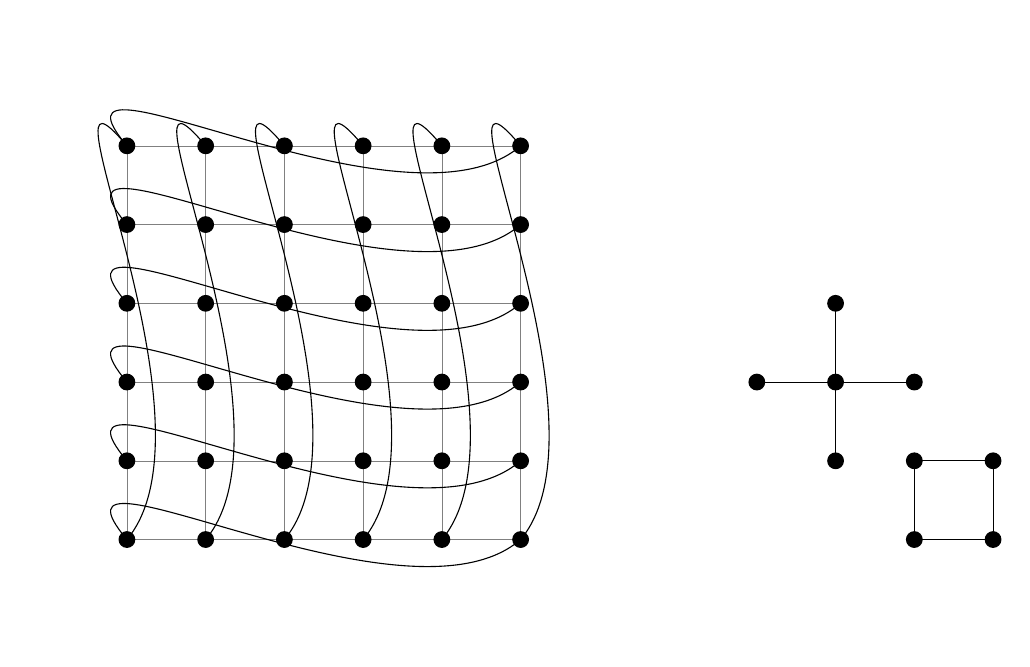
\begin{tikzpicture}
  \draw[step=1cm,gray,very thin] (0,0) grid (5,5);
  \foreach \x in {0,1,2,3,4,5}
  \foreach \y in {0,1,2,3,4,5}
  {
  \node[draw,circle,inner sep=2pt,fill] at (\x,\y) {};
}
\draw[ -> ]  (0,0) to [out=50, in=130] (0,5);
\draw[ -> ]  (1,0) to [out=50, in=130] (1,5);
\draw[ -> ]  (2,0) to [out=50, in=130] (2,5);
\draw[ -> ]  (3,0) to [out=50, in=130] (3,5);
\draw[ -> ]  (4,0) to [out=50, in=130] (4,5);
\draw[ -> ]  (5,0) to [out=50, in=130] (5,5);
\draw[ -> ]  (0,5) to [out=130, in=220] (5,5);
\draw[ -> ]  (0,4) to [out=130, in=220] (5,4);
\draw[ -> ]  (0,3) to [out=130, in=220] (5,3);
\draw[ -> ]  (0,2) to [out=130, in=220] (5,2);
\draw[ -> ]  (0,1) to [out=130, in=220] (5,1);
\draw[ -> ]  (0,0) to [out=130, in=220] (5,0);

\node[draw,circle,inner sep=2pt,fill] at (9,2) {};
\node[draw,circle,inner sep=2pt,fill] at (10,2) {};
\node[draw,circle,inner sep=2pt,fill] at (8,2) {};
\node[draw,circle,inner sep=2pt,fill] at (9,1) {};
\node[draw,circle,inner sep=2pt,fill] at (9,3) {};
\draw[ -> ]  (9,2) to (10,2);
\draw[ -> ]  (9,2) to (8,2);
\draw[ -> ]  (9,2) to (9,1);
\draw[ -> ]  (9,2) to (9,3);
%\draw[ -> ]  (9,2) to (5,0);

\node[draw,circle,inner sep=2pt,fill] at (10,1) {};
\node[draw,circle,inner sep=2pt,fill] at (11,1) {};
\node[draw,circle,inner sep=2pt,fill] at (10,0) {};
\node[draw,circle,inner sep=2pt,fill] at (11,0) {};
\draw[ -> ]  (10,1) to (11,1);
\draw[ -> ]  (10,1) to (10,0);
\draw[ -> ]  (10,0) to (11,0);
\draw[ -> ]  (11,1) to (11,0);
\end{tikzpicture}
\caption{On the left is the Toric Graph. On the right are cross and face checks.}
\label{fig:Toric}
\end{figure}
\end{center}
For example consider some vertex $v$ on the Torus, and let $\ket{\psi} = \sum_{x}{ \ket{\cdots x_{e_0}x_{e_1}x_{e_2}x_{e_3}  \cdots}}$ when $e_{0},e_{1},e_{2},e_{3}$ are the edges compose the local view of $v$. Then in any ket can be in the support of $\ket{\psi}$ only if the parity of $e_{0},e_{1},e_{2},e_{3}$ is even.
%\subsection{Note on the Toric in the presence of noise.} 

\begin{claim}
  The $l \times l$  Toric code is a CSS code, with dimension $2$ and distance $\Theta\left( l \right)$.   
\end{claim}
\begin{proof}
  Consider a pair of cross and a face checks. If they are not intersect (share edges) then, obviously, they commute. So suppose they share an edge. Now there are a finite number of cases ($4$) in which a cross check can intersect a face, and for all of them we have they must to intersect in an exactly two edges. Therefore the crosses checks commute with all the faces checks. 

  Now, denote by $C_{X}$ and $C_{Z}$ the linear codes defined by the crosses and faces checks. Observes that $C_{X}$ contain all the subgraph of the tours which have only evens degree, namely all the loops. The following claim will be used to show that all the low weight loops (squeezable loops) are in $C_{Z}^{\perp}$. 
  \begin{claim}
    Let $c$ be an assignment of ones on a unite square, namely a closed loop at length $4$, then $c \in C_{Z}^{\perp}$.  
  \end{claim}
  \begin{proof}
    Denote by $c^{\prime}$ a codeword of $C_{Z}$, therefore the parity sum induced by $c^{\prime}$ on any square equals zero, Particularly the induced parity on the square supporting $c$ is zero. But that parity is exactly $c\cdot c^{\prime}$. As it true for any $c^{\prime} \in C_{Z}$ we obtain that $c \in C_{Z}^{\perp}$.  
  \end{proof}
  \begin{claim}[Veblen's theorem]
    The set of even subgraph is a linear space spanned by simple cycles (vertices degree equals exactly 2).
  \end{claim}
  \begin{proof}
    Let $P \subset E$ be an even subgraph then it must to have a simple cycle denote it by $P^{\prime}$, now notice that $P/P^\prime$ is also an even subgraph. To see that consider a vertex $v$, As $P^{\prime}$ is simple cycle, substituting $P^{\prime}$ is either not effect the degree of $v$ in $P/P^{\prime}$ or it decrees $v$ degree by exactly $2$ so $d_{P/P^{\prime}}\left( v \right) = d_{P}\left( v \right) - 2$. In both cases $d_{P/P^{\prime}}\left( v \right)$ is even.
    By repeating recursively untill $P/P^{\prime} = \{ \emptyset \}$ we get a decomposition of $P$ into a sum of simple cycles.   
  \end{proof}

  \begin{claim}
    \label{claim:inter}
    Associate with any vertices of the Tours a coordinates in $\mathbb{Z}_{l} \times \mathbb{Z}_{l}$. Consider a simple cycle $P$ subset of the Torus. Denote $P$ by the vertices compose it $v_{0}v_{1}..v_{k}$ arranged by order. Consider a  vertex $v_{i} \in P$ such that $\{v_{i-1}, v_{i}\}$, $\{v_{i}, v_{i+1}\}$ are at the same direaction and denote $v = \left( x,y \right) \in $$ \mathbb{Z}_{l} \times \mathbb{Z}_{l}$. Then there exist vertex $u \in P$, $ u \neq v_{i-1}v_{i+1}$ that share one of the cordinates of $v$. Put it differnetly there exsit $z$ such either  $u = \left( z,y \right)$ or $u = \left( x,z \right)$. 
  \end{claim}

  \begin{proof}
  Assume without loose of genrality that $v_{i-1} = \left( x, y -1 \right)$ and $v_{i+1} =\left( x,y+1 \right)$. Now denote by $f$ the projection on the second cordinate, $f(a,b)= b$. and obseves that for any $j$ the distnace $f\left( v_{j+1}\right) - \left( v_{j}  \right)$ satisfies:
    \begin{equation*}
      \begin{split}
      f\left( v_{j+1}\right) - f \left( v_{j}  \right) = 
        \begin{cases}
          \pm \left( l - 1 \right)  & v_{j} = \left( \cdot, l -1 \right), v_{j+1} = \left( \cdot, 0  \right)  \\
          \in \{ \pm 1 , 0\} & \text{else}
        \end{cases}
      \end{split}
    \end{equation*}
    So if there is no $u \neq v_{i}$ such that $f(u) = f(v_{i}) = f(v_{i-1})+1$ then there must to be an edge $\{v_{j},v_{j+1}\}$, $v_{j} = \left( \cdot, l -1 \right)$, $ v_{j+1} = \left( \cdot, 0  \right)$ such $P$ pass trough it. So  
    \begin{equation*}
      \begin{split}
        f\left( v_{i-1} \right) & \le f\left( v+1 \right) +  |f\left( v+2 \right) -  f\left( v+1 \right)| + .. + -\left( l - 1 \right) \\ 
        & \le f(v+1) - |P| - \left(l-1\right)  
      \end{split}
    \end{equation*}
    But $|P| \le l$. 
  \end{proof}
  \begin{figure}[h]
 \begin{tikzpicture}
    \draw [thick, decorate, decoration={random steps,segment length=16pt,amplitude=1pt}]
 (1,0) to[out=90,in=90] (5,0);
    \draw [thick, decorate, decoration={random steps,segment length=16pt,amplitude=1pt}]
 (5,0) to[out=270,in=270] (1,-1);
    %\draw [thick, decorate, decoration={random steps,segment length=10pt,amplitude=2pt}]
 %(0,0) to[out=0,in=0] (0,4);
  \end{tikzpicture}
\end{figure}

  \begin{definition}
    Horizontal and Vertical diameters. Let $P$ be defined again as exactly as in cliam \cref{claim:inter}. We will say that the \textit{horizontial diameter} of $P$ is   
    \begin{equation*}
      \begin{split}
        \max_{v,u\in P} \min{ \left\{  | v_{x} -u_{x}|, |v_{x} + l + u_{x}| \right\} }  
      \end{split}
    \end{equation*}
    Similarly, we define the vertical diametr to be: 
    \begin{equation*}
      \begin{split}
        \max_{v,u\in P} \min{ \left\{  | v_{y} -u_{y}|, |v_{y} + l + u_{y}| \right\} }  
      \end{split}
    \end{equation*}
  \end{definition}

  \begin{claim} 
If $P$ is a non empty simple cycle with vertical and horizontal diameters $d_{1}, d_{2}$, then it can either be a square or can be decomposed into two simple cycles $P_{1},P^{2}$ with either the vertical diameter of both of them being strictly less than $d_{1}$ and their horizontal diameters being at most $d_{2}$, or the horizontal diameter of both of them being strictly less than $d_{2}$ and their vertical diameters being at most $d_{1}$.
  \end{claim}

  \begin{proof}
  \end{proof}

  \begin{claim}
  Any Simple cycle can be decmopise as sum of unite squares.     
  \end{claim}

  Let $c \in C_{X}$ at weight at most $l$ and by $G = (V,E)$ the Cayley graph of the tours, we will refer to each of the two generators of $G$ as directions. We will say that a tuple of edges $\{e_{1},e_{2}\}$ is corner of $c$ if they are both non zero coordinates of $c$ and in addition they match to different directions\footnote{On planner drawing, corner is just an horizontal edge followed by vertical edge}.        
 
  \begin{definition}
    Inner point.   If we draw a line than it intersect the shape odd number of times. Outer point, intersect even number of times.
  \end{definition}

  \begin{claim}
    Any simple cycle $P$ at length at most $l$, that is a subgraph of the $l \times l$ Torus can be emmbedd in  
  \end{claim}

  \begin{definition}
    Area of closed loop. The probability to pick an inner point. 
  \end{definition}

  \begin{claim}
    Let $c$ be a closed loop than there is a square $c^{\prime}$ such that $A(c + c^{\prime}) < A(c)$.
  \end{claim}

  \begin{proof}
  \end{proof}

\end{proof}

%The Toric code is a topological quantum error-correcting code that encodes a single qubit of information into a two-dimensional lattice of qubits. It is a stabilizer code, meaning that it uses a set of commuting operators to detect and correct errors. The code is based on the mathematical structure of a torus, and its properties make it a powerful tool for quantum computing. It is also a fault-tolerant code, meaning that it can correct errors even when some of the qubits are faulty.
%
%\begin{center}
%  \begin{tikzpicture}
%    \begin{tikzpicture}[scale=1.000000,x=1pt,y=1pt]
\filldraw[color=white] (0.000000, -7.500000) rectangle (240.000000, 217.500000);
% Drawing wires
% Line 1: a0 W
\draw[color=black] (0.000000,210.000000) -- (240.000000,210.000000);
% Line 2: b0 W
\draw[color=black] (0.000000,195.000000) -- (240.000000,195.000000);
% Line 3: c0 W
\draw[color=black] (0.000000,180.000000) -- (240.000000,180.000000);
% Line 4: d0 W
\draw[color=black] (0.000000,165.000000) -- (240.000000,165.000000);
% Line 5: e0 W
\draw[color=black] (0.000000,150.000000) -- (240.000000,150.000000);
% Line 6: a1 W
\draw[color=black] (0.000000,135.000000) -- (240.000000,135.000000);
% Line 7: b1 W
\draw[color=black] (0.000000,120.000000) -- (240.000000,120.000000);
% Line 8: c1 W
\draw[color=black] (0.000000,105.000000) -- (240.000000,105.000000);
% Line 9: d1 W
\draw[color=black] (0.000000,90.000000) -- (240.000000,90.000000);
% Line 10: e1 W
\draw[color=black] (0.000000,75.000000) -- (240.000000,75.000000);
% Line 11: a2 W
\draw[color=black] (0.000000,60.000000) -- (240.000000,60.000000);
% Line 12: b2 W
\draw[color=black] (0.000000,45.000000) -- (240.000000,45.000000);
% Line 13: c2 W
\draw[color=black] (0.000000,30.000000) -- (240.000000,30.000000);
% Line 14: d2 W
\draw[color=black] (0.000000,15.000000) -- (240.000000,15.000000);
% Line 15: e2 W
\draw[color=black] (0.000000,0.000000) -- (240.000000,0.000000);
% Done with wires; drawing gates
% Line 18: d0 C a0
\draw (9.000000,210.000000) -- (9.000000,165.000000);
\begin{scope}
\draw[fill=white] (9.000000, 165.000000) circle(3.000000pt);
\clip (9.000000, 165.000000) circle(3.000000pt);
\draw (6.000000, 165.000000) -- (12.000000, 165.000000);
\draw (9.000000, 162.000000) -- (9.000000, 168.000000);
\end{scope}
\filldraw (9.000000, 210.000000) circle(1.500000pt);
% Line 30: d1 C a1
\draw (9.000000,135.000000) -- (9.000000,90.000000);
\begin{scope}
\draw[fill=white] (9.000000, 90.000000) circle(3.000000pt);
\clip (9.000000, 90.000000) circle(3.000000pt);
\draw (6.000000, 90.000000) -- (12.000000, 90.000000);
\draw (9.000000, 87.000000) -- (9.000000, 93.000000);
\end{scope}
\filldraw (9.000000, 135.000000) circle(1.500000pt);
% Line 42: d2 C a2
\draw (9.000000,60.000000) -- (9.000000,15.000000);
\begin{scope}
\draw[fill=white] (9.000000, 15.000000) circle(3.000000pt);
\clip (9.000000, 15.000000) circle(3.000000pt);
\draw (6.000000, 15.000000) -- (12.000000, 15.000000);
\draw (9.000000, 12.000000) -- (9.000000, 18.000000);
\end{scope}
\filldraw (9.000000, 60.000000) circle(1.500000pt);
% Line 19: d0 C b0
\draw (27.000000,195.000000) -- (27.000000,165.000000);
\begin{scope}
\draw[fill=white] (27.000000, 165.000000) circle(3.000000pt);
\clip (27.000000, 165.000000) circle(3.000000pt);
\draw (24.000000, 165.000000) -- (30.000000, 165.000000);
\draw (27.000000, 162.000000) -- (27.000000, 168.000000);
\end{scope}
\filldraw (27.000000, 195.000000) circle(1.500000pt);
% Line 31: d1 C b1
\draw (27.000000,120.000000) -- (27.000000,90.000000);
\begin{scope}
\draw[fill=white] (27.000000, 90.000000) circle(3.000000pt);
\clip (27.000000, 90.000000) circle(3.000000pt);
\draw (24.000000, 90.000000) -- (30.000000, 90.000000);
\draw (27.000000, 87.000000) -- (27.000000, 93.000000);
\end{scope}
\filldraw (27.000000, 120.000000) circle(1.500000pt);
% Line 43: d2 C b2
\draw (27.000000,45.000000) -- (27.000000,15.000000);
\begin{scope}
\draw[fill=white] (27.000000, 15.000000) circle(3.000000pt);
\clip (27.000000, 15.000000) circle(3.000000pt);
\draw (24.000000, 15.000000) -- (30.000000, 15.000000);
\draw (27.000000, 12.000000) -- (27.000000, 18.000000);
\end{scope}
\filldraw (27.000000, 45.000000) circle(1.500000pt);
% Line 20: e0 C b0
\draw (45.000000,195.000000) -- (45.000000,150.000000);
\begin{scope}
\draw[fill=white] (45.000000, 150.000000) circle(3.000000pt);
\clip (45.000000, 150.000000) circle(3.000000pt);
\draw (42.000000, 150.000000) -- (48.000000, 150.000000);
\draw (45.000000, 147.000000) -- (45.000000, 153.000000);
\end{scope}
\filldraw (45.000000, 195.000000) circle(1.500000pt);
% Line 32: e1 C b1
\draw (45.000000,120.000000) -- (45.000000,75.000000);
\begin{scope}
\draw[fill=white] (45.000000, 75.000000) circle(3.000000pt);
\clip (45.000000, 75.000000) circle(3.000000pt);
\draw (42.000000, 75.000000) -- (48.000000, 75.000000);
\draw (45.000000, 72.000000) -- (45.000000, 78.000000);
\end{scope}
\filldraw (45.000000, 120.000000) circle(1.500000pt);
% Line 44: e2 C b2
\draw (45.000000,45.000000) -- (45.000000,0.000000);
\begin{scope}
\draw[fill=white] (45.000000, 0.000000) circle(3.000000pt);
\clip (45.000000, 0.000000) circle(3.000000pt);
\draw (42.000000, 0.000000) -- (48.000000, 0.000000);
\draw (45.000000, -3.000000) -- (45.000000, 3.000000);
\end{scope}
\filldraw (45.000000, 45.000000) circle(1.500000pt);
% Line 21: e0 C c0
\draw (63.000000,180.000000) -- (63.000000,150.000000);
\begin{scope}
\draw[fill=white] (63.000000, 150.000000) circle(3.000000pt);
\clip (63.000000, 150.000000) circle(3.000000pt);
\draw (60.000000, 150.000000) -- (66.000000, 150.000000);
\draw (63.000000, 147.000000) -- (63.000000, 153.000000);
\end{scope}
\filldraw (63.000000, 180.000000) circle(1.500000pt);
% Line 33: e1 C c1
\draw (63.000000,105.000000) -- (63.000000,75.000000);
\begin{scope}
\draw[fill=white] (63.000000, 75.000000) circle(3.000000pt);
\clip (63.000000, 75.000000) circle(3.000000pt);
\draw (60.000000, 75.000000) -- (66.000000, 75.000000);
\draw (63.000000, 72.000000) -- (63.000000, 78.000000);
\end{scope}
\filldraw (63.000000, 105.000000) circle(1.500000pt);
% Line 45: e2 C c2
\draw (63.000000,30.000000) -- (63.000000,0.000000);
\begin{scope}
\draw[fill=white] (63.000000, 0.000000) circle(3.000000pt);
\clip (63.000000, 0.000000) circle(3.000000pt);
\draw (60.000000, 0.000000) -- (66.000000, 0.000000);
\draw (63.000000, -3.000000) -- (63.000000, 3.000000);
\end{scope}
\filldraw (63.000000, 30.000000) circle(1.500000pt);
% Line 22: e0 G $X$
\begin{scope}
\draw[fill=white] (84.000000, 150.000000) +(-45.000000:8.485281pt and 8.485281pt) -- +(45.000000:8.485281pt and 8.485281pt) -- +(135.000000:8.485281pt and 8.485281pt) -- +(225.000000:8.485281pt and 8.485281pt) -- cycle;
\clip (84.000000, 150.000000) +(-45.000000:8.485281pt and 8.485281pt) -- +(45.000000:8.485281pt and 8.485281pt) -- +(135.000000:8.485281pt and 8.485281pt) -- +(225.000000:8.485281pt and 8.485281pt) -- cycle;
\draw (84.000000, 150.000000) node {$X$};
\end{scope}
% Line 34: d1 e1 +b1
\draw (84.000000,120.000000) -- (84.000000,75.000000);
\filldraw (84.000000, 90.000000) circle(1.500000pt);
\filldraw (84.000000, 75.000000) circle(1.500000pt);
\begin{scope}
\draw[fill=white] (84.000000, 120.000000) circle(3.000000pt);
\clip (84.000000, 120.000000) circle(3.000000pt);
\draw (81.000000, 120.000000) -- (87.000000, 120.000000);
\draw (84.000000, 117.000000) -- (84.000000, 123.000000);
\end{scope}
% Line 46: d2 e2 +b2
\draw (84.000000,45.000000) -- (84.000000,0.000000);
\filldraw (84.000000, 15.000000) circle(1.500000pt);
\filldraw (84.000000, 0.000000) circle(1.500000pt);
\begin{scope}
\draw[fill=white] (84.000000, 45.000000) circle(3.000000pt);
\clip (84.000000, 45.000000) circle(3.000000pt);
\draw (81.000000, 45.000000) -- (87.000000, 45.000000);
\draw (84.000000, 42.000000) -- (84.000000, 48.000000);
\end{scope}
% Line 23: d0 e0 +c0
\draw (108.000000,180.000000) -- (108.000000,150.000000);
\filldraw (108.000000, 165.000000) circle(1.500000pt);
\filldraw (108.000000, 150.000000) circle(1.500000pt);
\begin{scope}
\draw[fill=white] (108.000000, 180.000000) circle(3.000000pt);
\clip (108.000000, 180.000000) circle(3.000000pt);
\draw (105.000000, 180.000000) -- (111.000000, 180.000000);
\draw (108.000000, 177.000000) -- (108.000000, 183.000000);
\end{scope}
% Line 35: d1 G $X$
\begin{scope}
\draw[fill=white] (108.000000, 90.000000) +(-45.000000:8.485281pt and 8.485281pt) -- +(45.000000:8.485281pt and 8.485281pt) -- +(135.000000:8.485281pt and 8.485281pt) -- +(225.000000:8.485281pt and 8.485281pt) -- cycle;
\clip (108.000000, 90.000000) +(-45.000000:8.485281pt and 8.485281pt) -- +(45.000000:8.485281pt and 8.485281pt) -- +(135.000000:8.485281pt and 8.485281pt) -- +(225.000000:8.485281pt and 8.485281pt) -- cycle;
\draw (108.000000, 90.000000) node {$X$};
\end{scope}
% Line 47: d2 G $X$
\begin{scope}
\draw[fill=white] (108.000000, 15.000000) +(-45.000000:8.485281pt and 8.485281pt) -- +(45.000000:8.485281pt and 8.485281pt) -- +(135.000000:8.485281pt and 8.485281pt) -- +(225.000000:8.485281pt and 8.485281pt) -- cycle;
\clip (108.000000, 15.000000) +(-45.000000:8.485281pt and 8.485281pt) -- +(45.000000:8.485281pt and 8.485281pt) -- +(135.000000:8.485281pt and 8.485281pt) -- +(225.000000:8.485281pt and 8.485281pt) -- cycle;
\draw (108.000000, 15.000000) node {$X$};
\end{scope}
% Line 58: b1 G $H$
\begin{scope}
\draw[fill=white] (108.000000, 120.000000) +(-45.000000:8.485281pt and 8.485281pt) -- +(45.000000:8.485281pt and 8.485281pt) -- +(135.000000:8.485281pt and 8.485281pt) -- +(225.000000:8.485281pt and 8.485281pt) -- cycle;
\clip (108.000000, 120.000000) +(-45.000000:8.485281pt and 8.485281pt) -- +(45.000000:8.485281pt and 8.485281pt) -- +(135.000000:8.485281pt and 8.485281pt) -- +(225.000000:8.485281pt and 8.485281pt) -- cycle;
\draw (108.000000, 120.000000) node {$H$};
\end{scope}
% Line 61: b2 G $H$
\begin{scope}
\draw[fill=white] (108.000000, 45.000000) +(-45.000000:8.485281pt and 8.485281pt) -- +(45.000000:8.485281pt and 8.485281pt) -- +(135.000000:8.485281pt and 8.485281pt) -- +(225.000000:8.485281pt and 8.485281pt) -- cycle;
\clip (108.000000, 45.000000) +(-45.000000:8.485281pt and 8.485281pt) -- +(45.000000:8.485281pt and 8.485281pt) -- +(135.000000:8.485281pt and 8.485281pt) -- +(225.000000:8.485281pt and 8.485281pt) -- cycle;
\draw (108.000000, 45.000000) node {$H$};
\end{scope}
% Line 24: e0 G $X$
\begin{scope}
\draw[fill=white] (132.000000, 150.000000) +(-45.000000:8.485281pt and 8.485281pt) -- +(45.000000:8.485281pt and 8.485281pt) -- +(135.000000:8.485281pt and 8.485281pt) -- +(225.000000:8.485281pt and 8.485281pt) -- cycle;
\clip (132.000000, 150.000000) +(-45.000000:8.485281pt and 8.485281pt) -- +(45.000000:8.485281pt and 8.485281pt) -- +(135.000000:8.485281pt and 8.485281pt) -- +(225.000000:8.485281pt and 8.485281pt) -- cycle;
\draw (132.000000, 150.000000) node {$X$};
\end{scope}
% Line 36: d1 e1 +a1
\draw (132.000000,135.000000) -- (132.000000,75.000000);
\filldraw (132.000000, 90.000000) circle(1.500000pt);
\filldraw (132.000000, 75.000000) circle(1.500000pt);
\begin{scope}
\draw[fill=white] (132.000000, 135.000000) circle(3.000000pt);
\clip (132.000000, 135.000000) circle(3.000000pt);
\draw (129.000000, 135.000000) -- (135.000000, 135.000000);
\draw (132.000000, 132.000000) -- (132.000000, 138.000000);
\end{scope}
% Line 48: d2 e2 +a2
\draw (132.000000,60.000000) -- (132.000000,0.000000);
\filldraw (132.000000, 15.000000) circle(1.500000pt);
\filldraw (132.000000, 0.000000) circle(1.500000pt);
\begin{scope}
\draw[fill=white] (132.000000, 60.000000) circle(3.000000pt);
\clip (132.000000, 60.000000) circle(3.000000pt);
\draw (129.000000, 60.000000) -- (135.000000, 60.000000);
\draw (132.000000, 57.000000) -- (132.000000, 63.000000);
\end{scope}
% Line 56: c0 G $H$
\begin{scope}
\draw[fill=white] (132.000000, 180.000000) +(-45.000000:8.485281pt and 8.485281pt) -- +(45.000000:8.485281pt and 8.485281pt) -- +(135.000000:8.485281pt and 8.485281pt) -- +(225.000000:8.485281pt and 8.485281pt) -- cycle;
\clip (132.000000, 180.000000) +(-45.000000:8.485281pt and 8.485281pt) -- +(45.000000:8.485281pt and 8.485281pt) -- +(135.000000:8.485281pt and 8.485281pt) -- +(225.000000:8.485281pt and 8.485281pt) -- cycle;
\draw (132.000000, 180.000000) node {$H$};
\end{scope}
% Line 25: d0 e0 +b0
\draw (156.000000,195.000000) -- (156.000000,150.000000);
\filldraw (156.000000, 165.000000) circle(1.500000pt);
\filldraw (156.000000, 150.000000) circle(1.500000pt);
\begin{scope}
\draw[fill=white] (156.000000, 195.000000) circle(3.000000pt);
\clip (156.000000, 195.000000) circle(3.000000pt);
\draw (153.000000, 195.000000) -- (159.000000, 195.000000);
\draw (156.000000, 192.000000) -- (156.000000, 198.000000);
\end{scope}
% Line 37: d1 G $X$
\begin{scope}
\draw[fill=white] (156.000000, 90.000000) +(-45.000000:8.485281pt and 8.485281pt) -- +(45.000000:8.485281pt and 8.485281pt) -- +(135.000000:8.485281pt and 8.485281pt) -- +(225.000000:8.485281pt and 8.485281pt) -- cycle;
\clip (156.000000, 90.000000) +(-45.000000:8.485281pt and 8.485281pt) -- +(45.000000:8.485281pt and 8.485281pt) -- +(135.000000:8.485281pt and 8.485281pt) -- +(225.000000:8.485281pt and 8.485281pt) -- cycle;
\draw (156.000000, 90.000000) node {$X$};
\end{scope}
% Line 38: e1 G $X$
\begin{scope}
\draw[fill=white] (156.000000, 75.000000) +(-45.000000:8.485281pt and 8.485281pt) -- +(45.000000:8.485281pt and 8.485281pt) -- +(135.000000:8.485281pt and 8.485281pt) -- +(225.000000:8.485281pt and 8.485281pt) -- cycle;
\clip (156.000000, 75.000000) +(-45.000000:8.485281pt and 8.485281pt) -- +(45.000000:8.485281pt and 8.485281pt) -- +(135.000000:8.485281pt and 8.485281pt) -- +(225.000000:8.485281pt and 8.485281pt) -- cycle;
\draw (156.000000, 75.000000) node {$X$};
\end{scope}
% Line 49: d2 G $X$
\begin{scope}
\draw[fill=white] (156.000000, 15.000000) +(-45.000000:8.485281pt and 8.485281pt) -- +(45.000000:8.485281pt and 8.485281pt) -- +(135.000000:8.485281pt and 8.485281pt) -- +(225.000000:8.485281pt and 8.485281pt) -- cycle;
\clip (156.000000, 15.000000) +(-45.000000:8.485281pt and 8.485281pt) -- +(45.000000:8.485281pt and 8.485281pt) -- +(135.000000:8.485281pt and 8.485281pt) -- +(225.000000:8.485281pt and 8.485281pt) -- cycle;
\draw (156.000000, 15.000000) node {$X$};
\end{scope}
% Line 50: e2 G $X$
\begin{scope}
\draw[fill=white] (156.000000, -0.000000) +(-45.000000:8.485281pt and 8.485281pt) -- +(45.000000:8.485281pt and 8.485281pt) -- +(135.000000:8.485281pt and 8.485281pt) -- +(225.000000:8.485281pt and 8.485281pt) -- cycle;
\clip (156.000000, -0.000000) +(-45.000000:8.485281pt and 8.485281pt) -- +(45.000000:8.485281pt and 8.485281pt) -- +(135.000000:8.485281pt and 8.485281pt) -- +(225.000000:8.485281pt and 8.485281pt) -- cycle;
\draw (156.000000, -0.000000) node {$X$};
\end{scope}
% Line 57: a1 G $H$
\begin{scope}
\draw[fill=white] (156.000000, 135.000000) +(-45.000000:8.485281pt and 8.485281pt) -- +(45.000000:8.485281pt and 8.485281pt) -- +(135.000000:8.485281pt and 8.485281pt) -- +(225.000000:8.485281pt and 8.485281pt) -- cycle;
\clip (156.000000, 135.000000) +(-45.000000:8.485281pt and 8.485281pt) -- +(45.000000:8.485281pt and 8.485281pt) -- +(135.000000:8.485281pt and 8.485281pt) -- +(225.000000:8.485281pt and 8.485281pt) -- cycle;
\draw (156.000000, 135.000000) node {$H$};
\end{scope}
% Line 60: a2 G $H$
\begin{scope}
\draw[fill=white] (156.000000, 60.000000) +(-45.000000:8.485281pt and 8.485281pt) -- +(45.000000:8.485281pt and 8.485281pt) -- +(135.000000:8.485281pt and 8.485281pt) -- +(225.000000:8.485281pt and 8.485281pt) -- cycle;
\clip (156.000000, 60.000000) +(-45.000000:8.485281pt and 8.485281pt) -- +(45.000000:8.485281pt and 8.485281pt) -- +(135.000000:8.485281pt and 8.485281pt) -- +(225.000000:8.485281pt and 8.485281pt) -- cycle;
\draw (156.000000, 60.000000) node {$H$};
\end{scope}
% Line 26: d0 G $X$
\begin{scope}
\draw[fill=white] (180.000000, 165.000000) +(-45.000000:8.485281pt and 8.485281pt) -- +(45.000000:8.485281pt and 8.485281pt) -- +(135.000000:8.485281pt and 8.485281pt) -- +(225.000000:8.485281pt and 8.485281pt) -- cycle;
\clip (180.000000, 165.000000) +(-45.000000:8.485281pt and 8.485281pt) -- +(45.000000:8.485281pt and 8.485281pt) -- +(135.000000:8.485281pt and 8.485281pt) -- +(225.000000:8.485281pt and 8.485281pt) -- cycle;
\draw (180.000000, 165.000000) node {$X$};
\end{scope}
% Line 39: d1 e1 +c1
\draw (180.000000,105.000000) -- (180.000000,75.000000);
\filldraw (180.000000, 90.000000) circle(1.500000pt);
\filldraw (180.000000, 75.000000) circle(1.500000pt);
\begin{scope}
\draw[fill=white] (180.000000, 105.000000) circle(3.000000pt);
\clip (180.000000, 105.000000) circle(3.000000pt);
\draw (177.000000, 105.000000) -- (183.000000, 105.000000);
\draw (180.000000, 102.000000) -- (180.000000, 108.000000);
\end{scope}
% Line 51: d2 e2 +c2
\draw (180.000000,30.000000) -- (180.000000,0.000000);
\filldraw (180.000000, 15.000000) circle(1.500000pt);
\filldraw (180.000000, 0.000000) circle(1.500000pt);
\begin{scope}
\draw[fill=white] (180.000000, 30.000000) circle(3.000000pt);
\clip (180.000000, 30.000000) circle(3.000000pt);
\draw (177.000000, 30.000000) -- (183.000000, 30.000000);
\draw (180.000000, 27.000000) -- (180.000000, 33.000000);
\end{scope}
% Line 55: b0 G $H$
\begin{scope}
\draw[fill=white] (180.000000, 195.000000) +(-45.000000:8.485281pt and 8.485281pt) -- +(45.000000:8.485281pt and 8.485281pt) -- +(135.000000:8.485281pt and 8.485281pt) -- +(225.000000:8.485281pt and 8.485281pt) -- cycle;
\clip (180.000000, 195.000000) +(-45.000000:8.485281pt and 8.485281pt) -- +(45.000000:8.485281pt and 8.485281pt) -- +(135.000000:8.485281pt and 8.485281pt) -- +(225.000000:8.485281pt and 8.485281pt) -- cycle;
\draw (180.000000, 195.000000) node {$H$};
\end{scope}
% Line 27: d0 e0 +a0
\draw (204.000000,210.000000) -- (204.000000,150.000000);
\filldraw (204.000000, 165.000000) circle(1.500000pt);
\filldraw (204.000000, 150.000000) circle(1.500000pt);
\begin{scope}
\draw[fill=white] (204.000000, 210.000000) circle(3.000000pt);
\clip (204.000000, 210.000000) circle(3.000000pt);
\draw (201.000000, 210.000000) -- (207.000000, 210.000000);
\draw (204.000000, 207.000000) -- (204.000000, 213.000000);
\end{scope}
% Line 40: e1 G $X$
\begin{scope}
\draw[fill=white] (204.000000, 75.000000) +(-45.000000:8.485281pt and 8.485281pt) -- +(45.000000:8.485281pt and 8.485281pt) -- +(135.000000:8.485281pt and 8.485281pt) -- +(225.000000:8.485281pt and 8.485281pt) -- cycle;
\clip (204.000000, 75.000000) +(-45.000000:8.485281pt and 8.485281pt) -- +(45.000000:8.485281pt and 8.485281pt) -- +(135.000000:8.485281pt and 8.485281pt) -- +(225.000000:8.485281pt and 8.485281pt) -- cycle;
\draw (204.000000, 75.000000) node {$X$};
\end{scope}
% Line 52: e2 G $X$
\begin{scope}
\draw[fill=white] (204.000000, -0.000000) +(-45.000000:8.485281pt and 8.485281pt) -- +(45.000000:8.485281pt and 8.485281pt) -- +(135.000000:8.485281pt and 8.485281pt) -- +(225.000000:8.485281pt and 8.485281pt) -- cycle;
\clip (204.000000, -0.000000) +(-45.000000:8.485281pt and 8.485281pt) -- +(45.000000:8.485281pt and 8.485281pt) -- +(135.000000:8.485281pt and 8.485281pt) -- +(225.000000:8.485281pt and 8.485281pt) -- cycle;
\draw (204.000000, -0.000000) node {$X$};
\end{scope}
% Line 59: c1 G $H$
\begin{scope}
\draw[fill=white] (204.000000, 105.000000) +(-45.000000:8.485281pt and 8.485281pt) -- +(45.000000:8.485281pt and 8.485281pt) -- +(135.000000:8.485281pt and 8.485281pt) -- +(225.000000:8.485281pt and 8.485281pt) -- cycle;
\clip (204.000000, 105.000000) +(-45.000000:8.485281pt and 8.485281pt) -- +(45.000000:8.485281pt and 8.485281pt) -- +(135.000000:8.485281pt and 8.485281pt) -- +(225.000000:8.485281pt and 8.485281pt) -- cycle;
\draw (204.000000, 105.000000) node {$H$};
\end{scope}
% Line 62: c2 G $H$
\begin{scope}
\draw[fill=white] (204.000000, 30.000000) +(-45.000000:8.485281pt and 8.485281pt) -- +(45.000000:8.485281pt and 8.485281pt) -- +(135.000000:8.485281pt and 8.485281pt) -- +(225.000000:8.485281pt and 8.485281pt) -- cycle;
\clip (204.000000, 30.000000) +(-45.000000:8.485281pt and 8.485281pt) -- +(45.000000:8.485281pt and 8.485281pt) -- +(135.000000:8.485281pt and 8.485281pt) -- +(225.000000:8.485281pt and 8.485281pt) -- cycle;
\draw (204.000000, 30.000000) node {$H$};
\end{scope}
% Line 28: d0 G $X$
\begin{scope}
\draw[fill=white] (228.000000, 165.000000) +(-45.000000:8.485281pt and 8.485281pt) -- +(45.000000:8.485281pt and 8.485281pt) -- +(135.000000:8.485281pt and 8.485281pt) -- +(225.000000:8.485281pt and 8.485281pt) -- cycle;
\clip (228.000000, 165.000000) +(-45.000000:8.485281pt and 8.485281pt) -- +(45.000000:8.485281pt and 8.485281pt) -- +(135.000000:8.485281pt and 8.485281pt) -- +(225.000000:8.485281pt and 8.485281pt) -- cycle;
\draw (228.000000, 165.000000) node {$X$};
\end{scope}
% Line 54: a0 G $H$
\begin{scope}
\draw[fill=white] (228.000000, 210.000000) +(-45.000000:8.485281pt and 8.485281pt) -- +(45.000000:8.485281pt and 8.485281pt) -- +(135.000000:8.485281pt and 8.485281pt) -- +(225.000000:8.485281pt and 8.485281pt) -- cycle;
\clip (228.000000, 210.000000) +(-45.000000:8.485281pt and 8.485281pt) -- +(45.000000:8.485281pt and 8.485281pt) -- +(135.000000:8.485281pt and 8.485281pt) -- +(225.000000:8.485281pt and 8.485281pt) -- cycle;
\draw (228.000000, 210.000000) node {$H$};
\end{scope}
% Done with gates; drawing ending labels
% Done with ending labels; drawing cut lines and comments
% Line 64: a0 e0 @ 1 7
% Done with comments
\end{tikzpicture}

%  \end{tikzpicture}
%\end{center}

%\begin{algorithm}[H]
%  \caption{Shor code decoder.}
%    \label{alg:shordecoder}
%    \KwData{ $ \ket{\psi} \in \mathbb{C}_{2}^{9}$ }
%    \KwResult{ Correct a single fault. }
%    Let $D$ be a decoder for the classic repetition code over $3$ qubits. \\ 
%    Let $\ket{x_{1}x_{2}x_{3}} \leftarrow \ket{\psi}$ \\ 
%
%    $ L \leftarrow \text{Array} \{ \} $\\
%    \For { $ v \in V$} {
%      $c^{\prime}_{v} \leftarrow \arg\min {\left\{  y \in C_{0} : |y + x|_{v} |  \right\} } $\\
%      $ L_{v} \leftarrow c^{\prime}_{v}$
%    }
%    $ z \leftarrow \sum_{v \in V}{c^{\prime}_{v}} $\\
%    \eIf{ $ |z| < \tau \frac{n}{f\left( n \right)} $}{
%      \While{ $|z| > 0$ }{
%	find $v$ and $c \in C_{0}$ such that $|z + c_{v}| < |z|$\\
%	$z \leftarrow z + c_{v}$ \\
%	$ L_{v} \leftarrow  L_{v} + c_{v}$
%      }
%    }{
%      reject. 
%    }
%    \Return  $S(L) $
%
%  \end{algorithm}

%
%By quadric the dimension of the repetition code one can find those state which at least two pauli are needed to applay for flipping either the bit or the phase of the logic state. Clearly any phase flip 
 
\section{Quantum Expander Codes.}
%As similar to the classical case, the next natural question to ask is whether there are codes with positive rate. The quantum expanders were the first quantum LDPC codes to achieve a square root distance and positive rate \cite{Tillich_2014, Leverrier_2015}. The leading insight was the idea that the Toric code could be represented as a variant product of the repetition code.  For example, consider the cross restriction in figure \cref{fig:Toric}, that restriction can be obtained by gluing two vertices of two different cycle graphs. 
As similar to the classical case, the next natural question to ask is whether there are codes with positive rates. The quantum expanders were the first quantum LDPC codes to achieve a square-root distance and positive rate \cite{Tillich_2014, Leverrier_2015}. The leading insight was the idea that the Toric code could be represented as a variant product of the repetition code. For example, consider the cross restriction in Figure \cref{fig:Toric}; that restriction can be obtained by gluing two vertices of two different cycle graphs.

\begin{definition}
  For any two matrices $A,B$, with the same number of rows, denote by $\left[ A,B \right]$ the matrix obtained by attach $B$ next to $A$ from right.  Let $H_{1}, H_{2} \in \mathbb{F}_{2}^{n\times r}$ be the parity check matrices. Define the bit and the phase parity checks matrices to be:          
\begin{equation*}
  \begin{split}
    H_{X} &= \left[ H_{1} \otimes I_{r} \ \  I_{n} \otimes H^{\top}_{2} \right] \\ 
    H_{Z} &= \left[ I_{r} \otimes H_{2} \ \  H_{1}^{\top} \otimes I_{n} \right] \\ 
  \end{split}
  \label{equ:css}
\end{equation*}
The matrices are orthogonal to each other as $H_{X}H_{Z}^{\top} = H_{1}\otimes H^{\top}_{2} + H_{1}\otimes H^{\top}_{2} = 0$ and therefore the pair define a valid CSS code. We will call to that code the Hyperproduct and denote it by $Q\left( H_{1} \times H_{2} \right)$.
\end{definition}
Obliviously, if $H_{1},H_{2},H_{1}^{\top},H_{2}^{\top}$ are parity checks matrices of an LDPC codes, so are $H_{X},H_{Z}$ as their maximal row weight is at most two times larger.   
%\ref{equ:css}

% That insight raise the following perspective. The Toric code could be thought as tanner code defined on product of two cycles. If the checks in the repetition code are of the form $H_i =  x_i + x_{i+1}$  then in the Toric code the checks are $x_{i,j}+ x_{i, j+1} + x_{i+1, j} + x_{i+1,j+1}$. Namely any restriction over the edge in the Toric code  $x_{e_{0}}+ x_{e_{1}} + x_{e_{2}} + x_{e_{3}} = 0$ is obtained by taking two restrictions of the repetition code and multiple them.

\begin{sagesilent}
latex.matrix_delimiters('[', ']')
M = matrix(GF(2), [1 for _ in range(3)])
repetition = codes.LinearCode(M)
H = repetition.parity_check_matrix().stack( matrix(GF(2), [1,1,0]))
H1 = identity_matrix(3).tensor_product(H).augment( H.transpose().tensor_product(identity_matrix(3)))
Hstr = latex(H)
H1str = latex(H1)
\end{sagesilent}

\begin{example}
  The Toric code could be thought as the Hyperproduct of the repetition code with himself. The parity check matrices of the codes are given follow. The left $3 \times 3$ matrix corresponds to the repetition code while the right $18 \times  9$ corresponds to the vertices check of the Toric code.  
\end{example}

\begin{equation*}
  \begin{split}
    \sagestr{Hstr} \sagestr{H1str} 
  \end{split}
\end{equation*}


\begin{claim}
  \label{claim:kerdim}
  Let  $A,B \in \mathbb{M}_{n\times r_{1}}, \mathbb{M}_{n\times r_{2}}$ then  $\dim \ker [A ,B]$ is $ \dim \ker A + n $. 
\end{claim}

\begin{proof}
  The proof is omitted. 
\end{proof}

\begin{claim}
  Let $k_{1},k_{2}$ be the demission of the codes with the full rank  parity check matrices $H_{1},H_{2}$. Then the dimension of the Hyperproduct code is $ \ge k_{1}k_{2}$. 
\end{claim}

\begin{proof}
  %We will find the dimensions of each of the classics codes defined by $H_{X}$ and $H_{Z}$. Notice that length of the code, assuming the fullness of the ranks, is $n^{2} +  (n-k_{1}) \cdot \left( n -k_{2}\right)$. Note that for any $u,v$ such $H_{1}u = 0$ and $H_{2}^{\top}v =0$ it holds that $[u\otimes e_{i} \ e_{j}\otimes v]$ is a codeword, where $e_{i},e_{j}$ are taken from the standard basis of $[n],[n-k_{2}]$. Thus the dimension of $\ker H_{X}$ is $k_{1}n + (n-k_{1})(n-k_{2})$. 
  %By the same arguments we have that $\dim C_{Z} = k_{2}n + (n-k_{1})(n-k_{2})$. 

  We will find the dimensions of each of the classical codes defined by $\ker H_{X}$ and $ \ker H_{Z}$. Notice that the length of the $H \otimes I_{n}$ equals $n\times n = n^2$, And  assuming the fullness of the ranks, the length of $ I_{r_{1}} \otimes  H_{2}^{\top} $  is $ r_{1}\cdot r_{2}$. Thus the length of $ \ker H_{X}$ is  $n^{2} + r_{1}r_{2}$ 
  %(n-k_{1}) \cdot \left( n -k_{2}\right)$. 
  Now, recall that for any matrix $A$ it holds that $\dim \ker \left( A \otimes I_{l} \right) = l \cdot \dim \ker A$. Therefore using \cref{claim:kerdim} we obtain that the dimension of $\ker H_{X}$ is $k_{1}n + r_{1}r_{2}$ 
  %(n-k_{1})(n-k_{2})$. Using  

  By the same arguments we have that $\dim C_{Z} = k_{2}n + r_{1}r_{2}$ % (n-k_{1})(n-k_{2})$.
Thus the dimension of the quantum code is:
  \begin{equation*}
    \begin{split}
      \dim Q\left( C_{X}, C_{Z} \right) &= \dim C_{X} + \dim C_{Z} - \left(  n^{2} + (n-k_{1})(n-k_{2})  \right) \\ 
      & = \left( k_{1} + k_{2} \right)n + 2(n-k_{1})(n-k_{2}) -\left(  n^{2} +  (n-k_{1}) \cdot \left( n -k_{2}\right) \right) \\
      & =k_{1}k_{2} 
    \end{split}
  \end{equation*}
\end{proof}

\begin{remark}
  \label{remark:pun}
  Let $H_{1}^{\prime}$ be a parity check matrix obtained by puncturing columns from $H_{1}$, denote by $k^{\prime}_{1}$ the dimension of that code. Then the Hyperproduct $Q(H_{1}^{\prime}\times H_{2})$ is a CSS code with dimension $k^{\prime}_{1}k_{2}$. Moreover if the number of columns left after the puncturing is less the distance of $\ker H_{1}$ then it must to holds that $k^{\prime}_{1} = 0 \Rightarrow \dim Q(H_{1}^{\prime} \times H_{2}) = 0$. Otherwise, one can take a non trivial codeword of $\ker H^{\prime}_{1}$ and extending it to a valid codeword of $\ker H_{1}$ by set any punctured coordinate of it to zero. The yielded codeword has weight less than $d$ which is contradiction.  
\end{remark}

\begin{claim}
  \label{claim:Hdis}
  Denote by $d$ the minimal distance of $\ker H_{1}$. Any codeword $x$ of $C_{X} = \ker H_{X}$ with edge at most $d$ belongs to $C_{Z}^{\perp}$.  
\end{claim}

\begin{proof}
  Define by $H^{\prime}_{1}$ the matrix which obtained by puncturing from $H_{1}$ the columns  associated with the coordinates $e_{i}$ such that subspace corresponding to $ e_{i} \otimes I_{n} $ doesn't support $x$. Denote the by $S$ the set of the reaming coordinates.  For example if $ H_{1} \otimes I_{n} = I_{2} \otimes I_{2}$ and $x = [1,0,0,0]$ then $H^{\prime}_{1} $ is the unit matrix $[1 , 0]^\top$ obtained by puncturing the second column of $H_{1} = I_{2}$, and $S= \{ e_{1} \} $ .  


  As $|x| < d $ we have that $|S| < d$, Namely $H^{\prime}_{1}$ supported on less than $d$ coordinates and therefore $\dim Q\left( H^{\prime}_{1} \times H_{2} \right)= k^{\prime}_{1}k_{2} = 0$.  Thus, by the fact that for any CSS code $\dim C = \dim C_{X} - \dim C_{Z}^\perp$ it follows that $\dim \ker H_{X}^{\prime}  = \dim \ker H_{Z}^{\prime \perp}$ $ \Rightarrow \ker H_{X}^{\prime}  = \ker H_{Z}^{\prime \perp}$.  Denote by $x^{\prime}$ the restriction of $x$ to the columns of $H_{X}^{\prime}$ and clearly, by the definition of the construction,  $x^{\prime}$ is a codeword of $\ker H_{X}^{\prime}$. Thus $x^{\prime}$ is also codeword of $\ker H_{Z}^{\prime \perp}$ and by the same argument, $x$ is also a codeword of $\ker H_{Z}^{\prime \perp}$. 
\end{proof}

Immediately from \cref{claim:Hdis} we obtain that existences of quantum LDPC codes with positive rate and $\Theta\left( \sqrt{n} \right)$ distance by taking the Hyperproduct of two classical expender codes.   

\begin{theorem}
  There exists an infinity family of QLDPC codes with positive rate and $\Theta(\sqrt{n})$ distance.   
\end{theorem}

%\section{Quantum Codes.}
%\begin{definition}
%  A $\left[\left[ n,k,d \right]\right]$ is a quantum code over $n$ qubits, that encode a subspace at demission $k$ and any fault composed by a product of at most $d/2$ Pauli operators. 
%\end{definition}
%



%\printbibliography[heading=subbibliography]

